\chapter{Implementation}
\label{chap:implementation}
In this chapter, we present and discuss our methods for analyzing basins and basin boundaries.

\section{Accessible region}
In order to construct and analyze the basin map and basin boundary, we need to reduce the dimension of the phase space, which is 8-dimensional. As our space time is stationary and has axial symmetry, the coordinates $t$ and $\phi$ can be dropped. In Weyl-cylindrical coordinates for stationary and axial symmetric space-times, we can write $\xi^\mu_{(t)} = \delta^\mu_t$ and $\xi^\mu_{(\phi)} = \delta^\mu_\phi$. From \eqref{eq:killings} we obtain $u^t = -\frac{\epsilon}{g_{tt}}$, where $g_{tt} = g_{tt}(\rho,z)$. The same can be done for $u^{\phi}$. Hence, we end up with $u^t = u^t(\rho, z), u^\phi = u^\phi(\rho,z)$. Now we reduce our phase space to $(\rho,u^\rho,z, u^z)$.

From normalization of the four-velocity, we have the following

\begin{equation}
    -1 = g_{\mu\nu}u^{\mu}u^{\nu} = \epsilon^2g^{tt}+l^2g^{\phi\phi} + g_{\rho\rho}[(u^\rho)^2+(u^z)^2].
    \label{eq:normalization}
\end{equation}

Thus, we can have $u^z = u^z(\rho,z,u^\rho)$. Further reduction can be done by fixing the $z$ coordinate or by expressing $z$ as a function of the $\rho$ coordinate, $z=z(\rho).$ Unless otherwise indicated, we will fix the $z$ coordinate. 

In the resulting 2-dimensional phase space $(\rho,u^\rho)$, the accessible region is constrained by the maximal value of $u^\rho$. The maximum value of $u^\rho$ denoted as $u^\rho_{MAX}$ is when $u^z=0$. From normalization~\eqref{eq:normalization} we obtain the following result.

\begin{equation}
    u^\rho_{MAX} = \pm \sqrt{\frac{-1-\epsilon^2g^{tt}-l^2g^{\phi\phi}}{g_{\rho\rho}}},
    \label{eq:urhomax}
\end{equation}

or equivalently

\begin{equation}
    u^\rho_{MAX} = \pm \sqrt{
    -g^{\rho\rho}- \epsilon^2g^{tt}g^{\rho\rho}-l^2g^{\phi\phi}g^{\rho\rho}},
    \label{eq:urhomax2}
\end{equation}

where we used $g^{\mu\nu} = \frac{1}{g_{\mu\nu}}$. As in $g^{\rho\rho} >0$, this gives us a condition

\begin{equation}
    -g^{tt}( \epsilon^2+g_{tt}+l^2g^{\phi\phi}g_{tt})\geq0.
    \label{eq:accessibleregioncondition}
\end{equation}

Since $\epsilon$ represents the conserved energy, we can define $V_{ef} \coloneqq -(g_{tt}+l^2g^{\phi\phi}g_{tt})$.

The accessible region is therefore constrained by $u^\rho_{MAX}$ and only the initial conditions for $u^\rho$ are possible that satisfy $|u^\rho|\leq|u^\rho_{MAX}|$. In the numerical implementation, we will reduce the computation to the $u^\rho \geq 0$ part of the phase space.

\subsection{Schwarzschild--Bach--Weyl system}
For the Schwarzschild black hole with a Bach--Weyl ring, which we abbreviate as the SCHW+BW system, we want to analyze when the test particle can escape to infinity. We will simply take the limit of \eqref{eq:accessibleregioncondition} as $\rho \rightarrow\infty$. Before that, we will evaluate the limits of $\nu_{\mathrm{Schw}}$ and $\nu_{\mathrm{BW}}$ as $\rho \rightarrow \infty$. As $\rho \rightarrow \infty$, $k^2 \rightarrow0$, the elliptic integral $K(k)$ therefore approaches some constant value and both \(\nu_{\mathrm{Schw}}\) and \(\nu_{\mathrm{BW}}\) tend to zero. Therefore, the limit of \eqref{eq:accessibleregioncondition} is $\epsilon^2 \geq 1$. Since geodesics are time-like, we have $\epsilon>0$ and get the energy constraints for the outcomes. Escape to infinity is possible if and only if $\epsilon \geq1$. In this thesis, we will analyze only scenarios with $\epsilon<1$, therefore only scenarios with two outcomes, either eternal orbit or collision with the black hole or the ring. 

\subsection{Reissner--Nordstr\"om--Majumdar--Papapetrou system}
As noted by Polcar, Sukova and Semerak~\cite{Polcar2019}, in the case of the Reissner--Nordstr\"om black hole with a Majumdar--Papapetrou ring, which we abbreviate as the RN+MP system, the accessible regions tend to be closed, whereas in the SCHW+BW system they often open towards the horizon. Therefore, we need to analyze if it is possible for a test particle in the RN+MP space-time to fall into the black hole. The effective potential for the RN+MP system reads

\begin{equation}
    V_{\mathrm{ef}} = \frac{l^2}{\rho^2}N^4+N^2,
\end{equation}

where
\begin{equation}
    N
    =
    \frac{1}{
    1+\frac{M}{\sqrt{\rho^2+z^2}}
    +\frac{2\mathcal{M}K(k)}{\pi l_2}}.
\end{equation}
For fixed \(z\neq0\), \(N\) has a finite nonzero limit as
\(\rho\rightarrow0^+\), and the centrifugal term
\(l^2N^4/\rho^2\) diverges. The accessible region therefore does not open
towards the horizon along such a fixed-\(z\) section. To obtain initial
conditions that can approach the horizon in the reduced
\((\rho,u^\rho)\) plane, we let \(z\) approach zero together with \(\rho\).
The path used in the numerical calculations is
\(z=z(\rho)=n\sqrt{M\rho}\), which gives
\(\sqrt{\rho^2+z^2}\sim |n|\sqrt{M\rho}\) near the horizon. Along this path,
\(N\sim |n|\sqrt{\rho/M}\), so

\begin{equation}
    \lim_{\rho \rightarrow 0^+} \frac{l^2}{\rho^2}N^4
    =
    \frac{l^2n^4}{M^2}.
\end{equation}

The allowed-region condition is \(\epsilon^2\geq V_{\mathrm{ef}}\). Hence,
near the horizon on this path the necessary limiting condition is

\begin{equation}
    \epsilon^2 \geq \frac{l^2n^4}{M^2}.
    \label{eq:rnmpcondition}
\end{equation}

By calculating the limit of the effective potential with $z=z(\rho)$ as $\rho \rightarrow \infty$, we end up with the same condition to escape to infinity as for the SCHW+BW system.

For fixed \(z\), the effective potential diverges as \(\rho\rightarrow0^+\), as
shown in Figure~\ref{fig:rn-mp-veff-fixed-z}.

\begin{figure}[H]
    \centering
    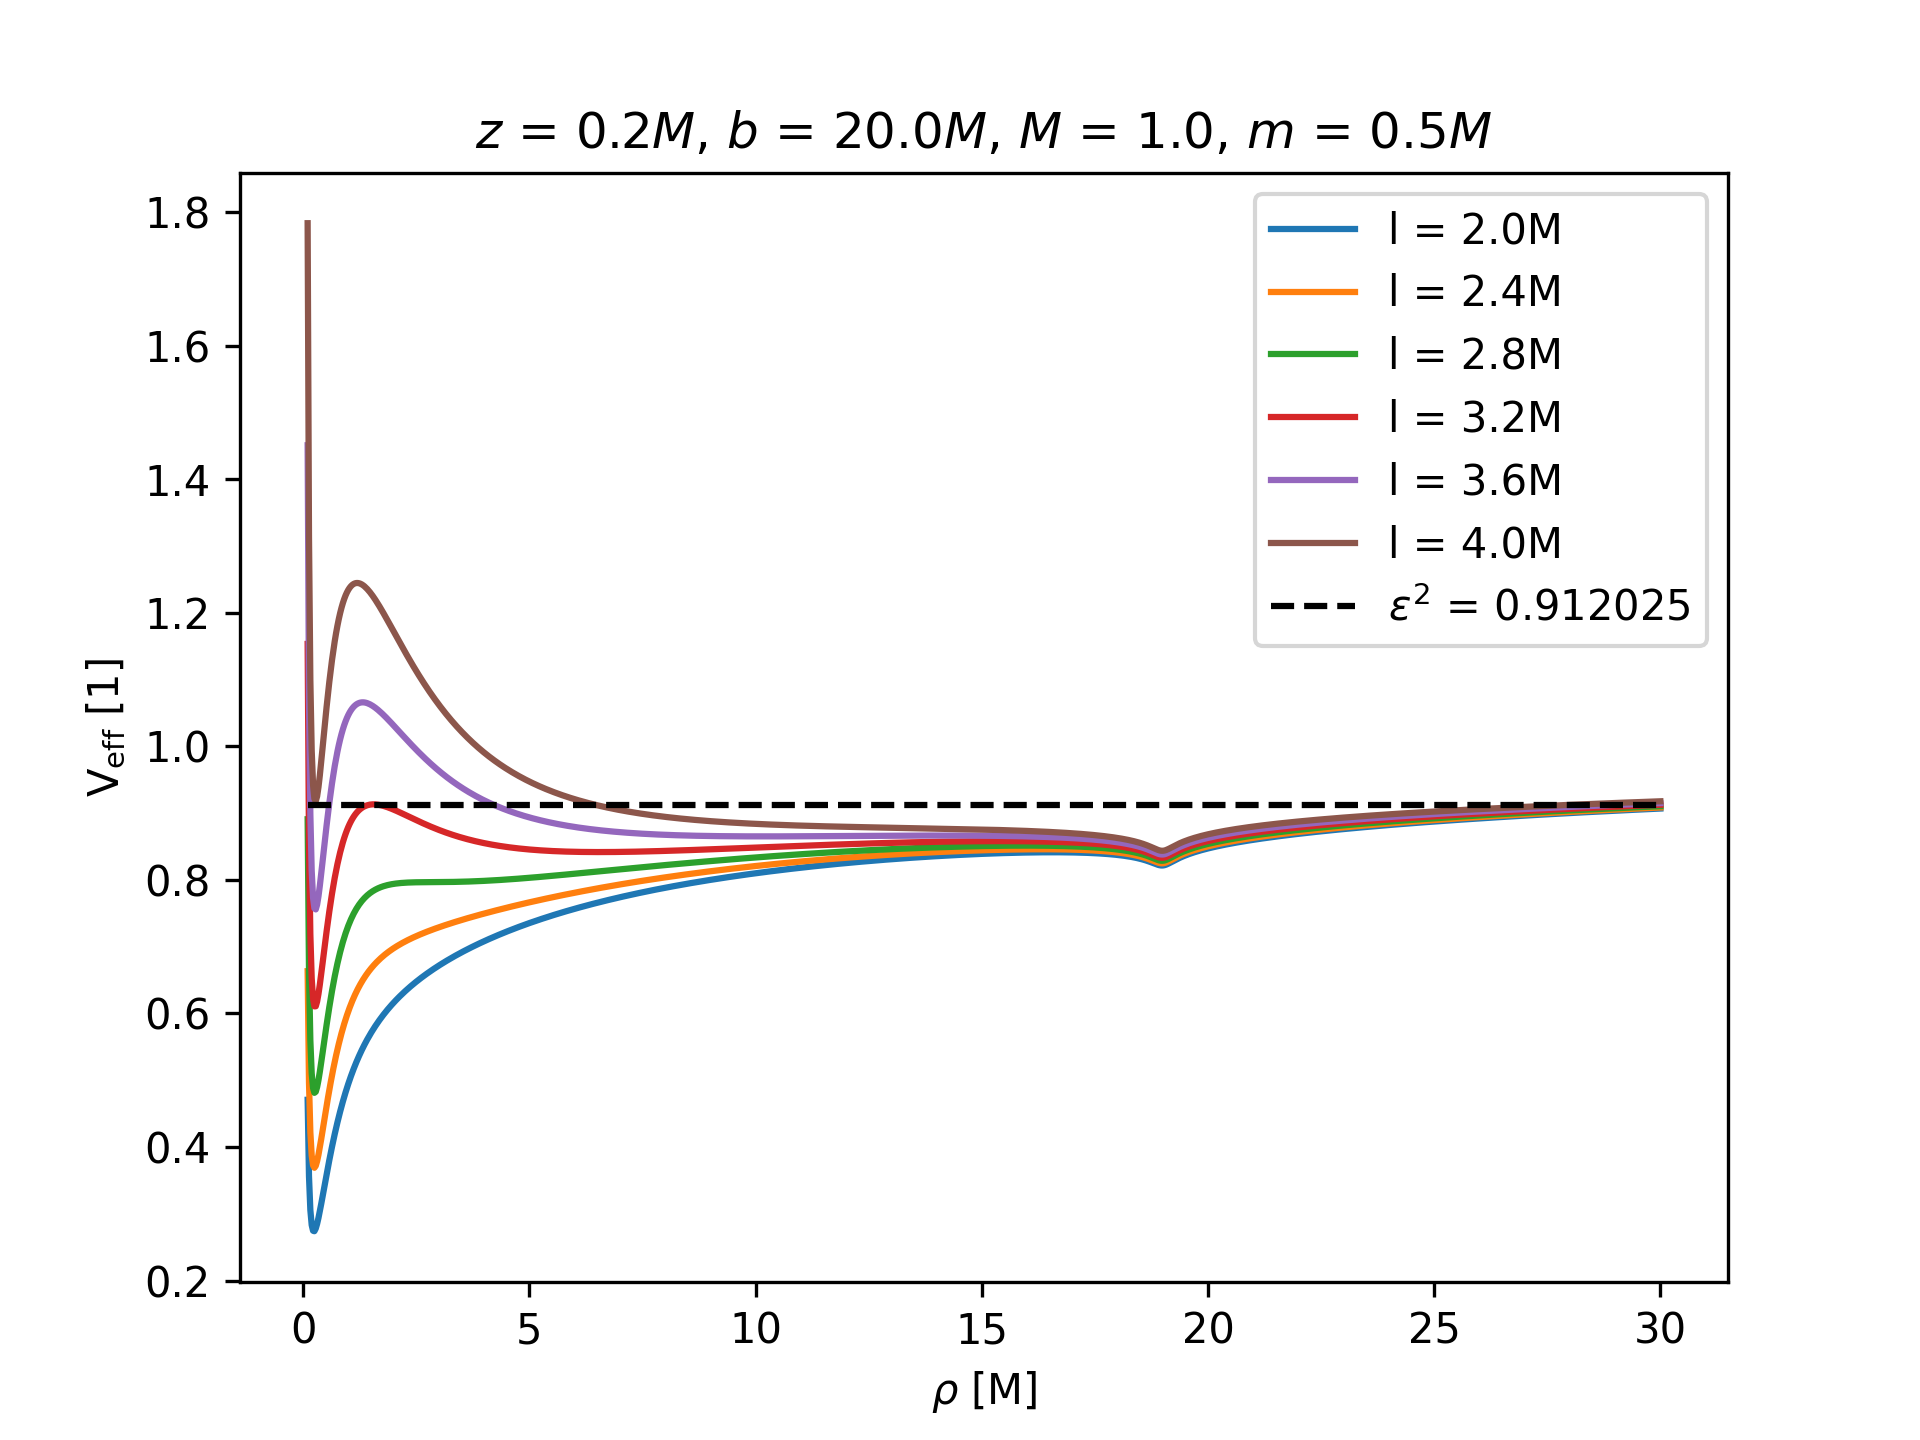
\includegraphics[width=0.82\linewidth]{img/rn_mp_Veff_fix_z.png}
    \caption{Effective potential \(V_{\mathrm{ef}}\) of the Reissner--Nordstr\"om--Majumdar--Papapetrou (RN+MP) system for fixed \(z=0.2M\), \(M=1\), \(\mathcal{M}=0.5M\), \(b=20M\), and several values of the angular momentum \(l\). The horizontal dashed line marks \(\epsilon^2\) for \(\epsilon=0.955\).}
    \label{fig:rn-mp-veff-fixed-z}
\end{figure}

This results in an accessible region not opening towards the horizon. 

\begin{figure}[H]
    \centering
    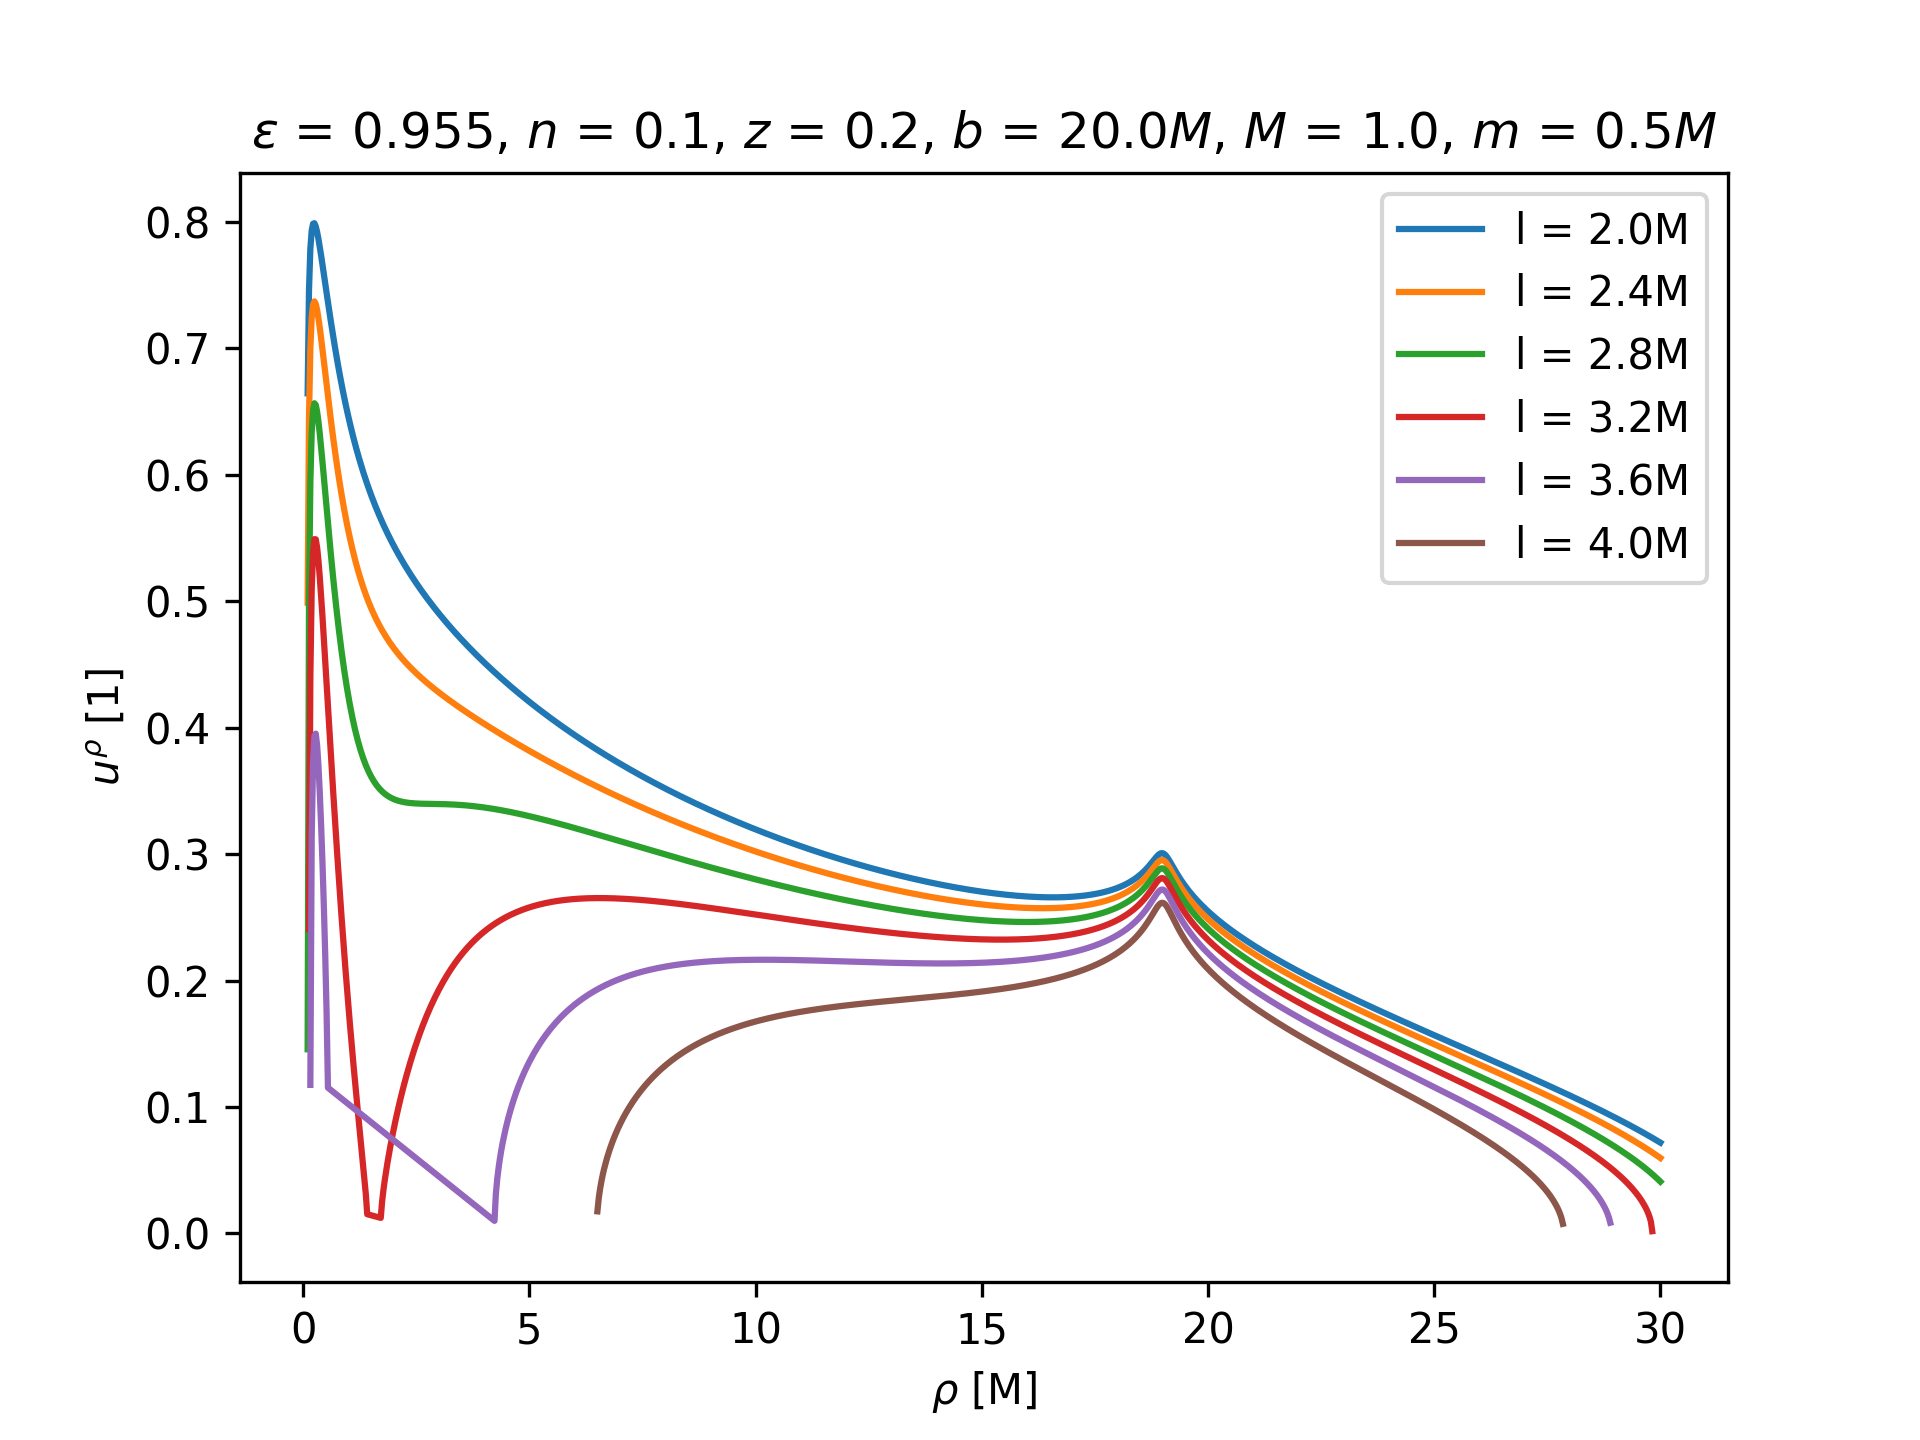
\includegraphics[width=0.82\linewidth]{img/rn_mp_accessible_region_fix_z.png}
    \caption{Accessible region of the RN+MP system for fixed \(z=0.2M\), \(M=1\), \(\mathcal{M}=0.5M\), \(b=20M\), \(\epsilon=0.955\), and several values of \(l\). The plotted curves give the positive branch of \(u^\rho_{\mathrm{MAX}}\).}
    \label{fig:rn-mp-accessible-fixed-z}
\end{figure}

Now consider \(z=z(\rho)\) and the condition~\eqref{eq:rnmpcondition}. The corresponding effective potential and accessible region are shown in the next two figures. 

\begin{figure}[H]
    \centering
    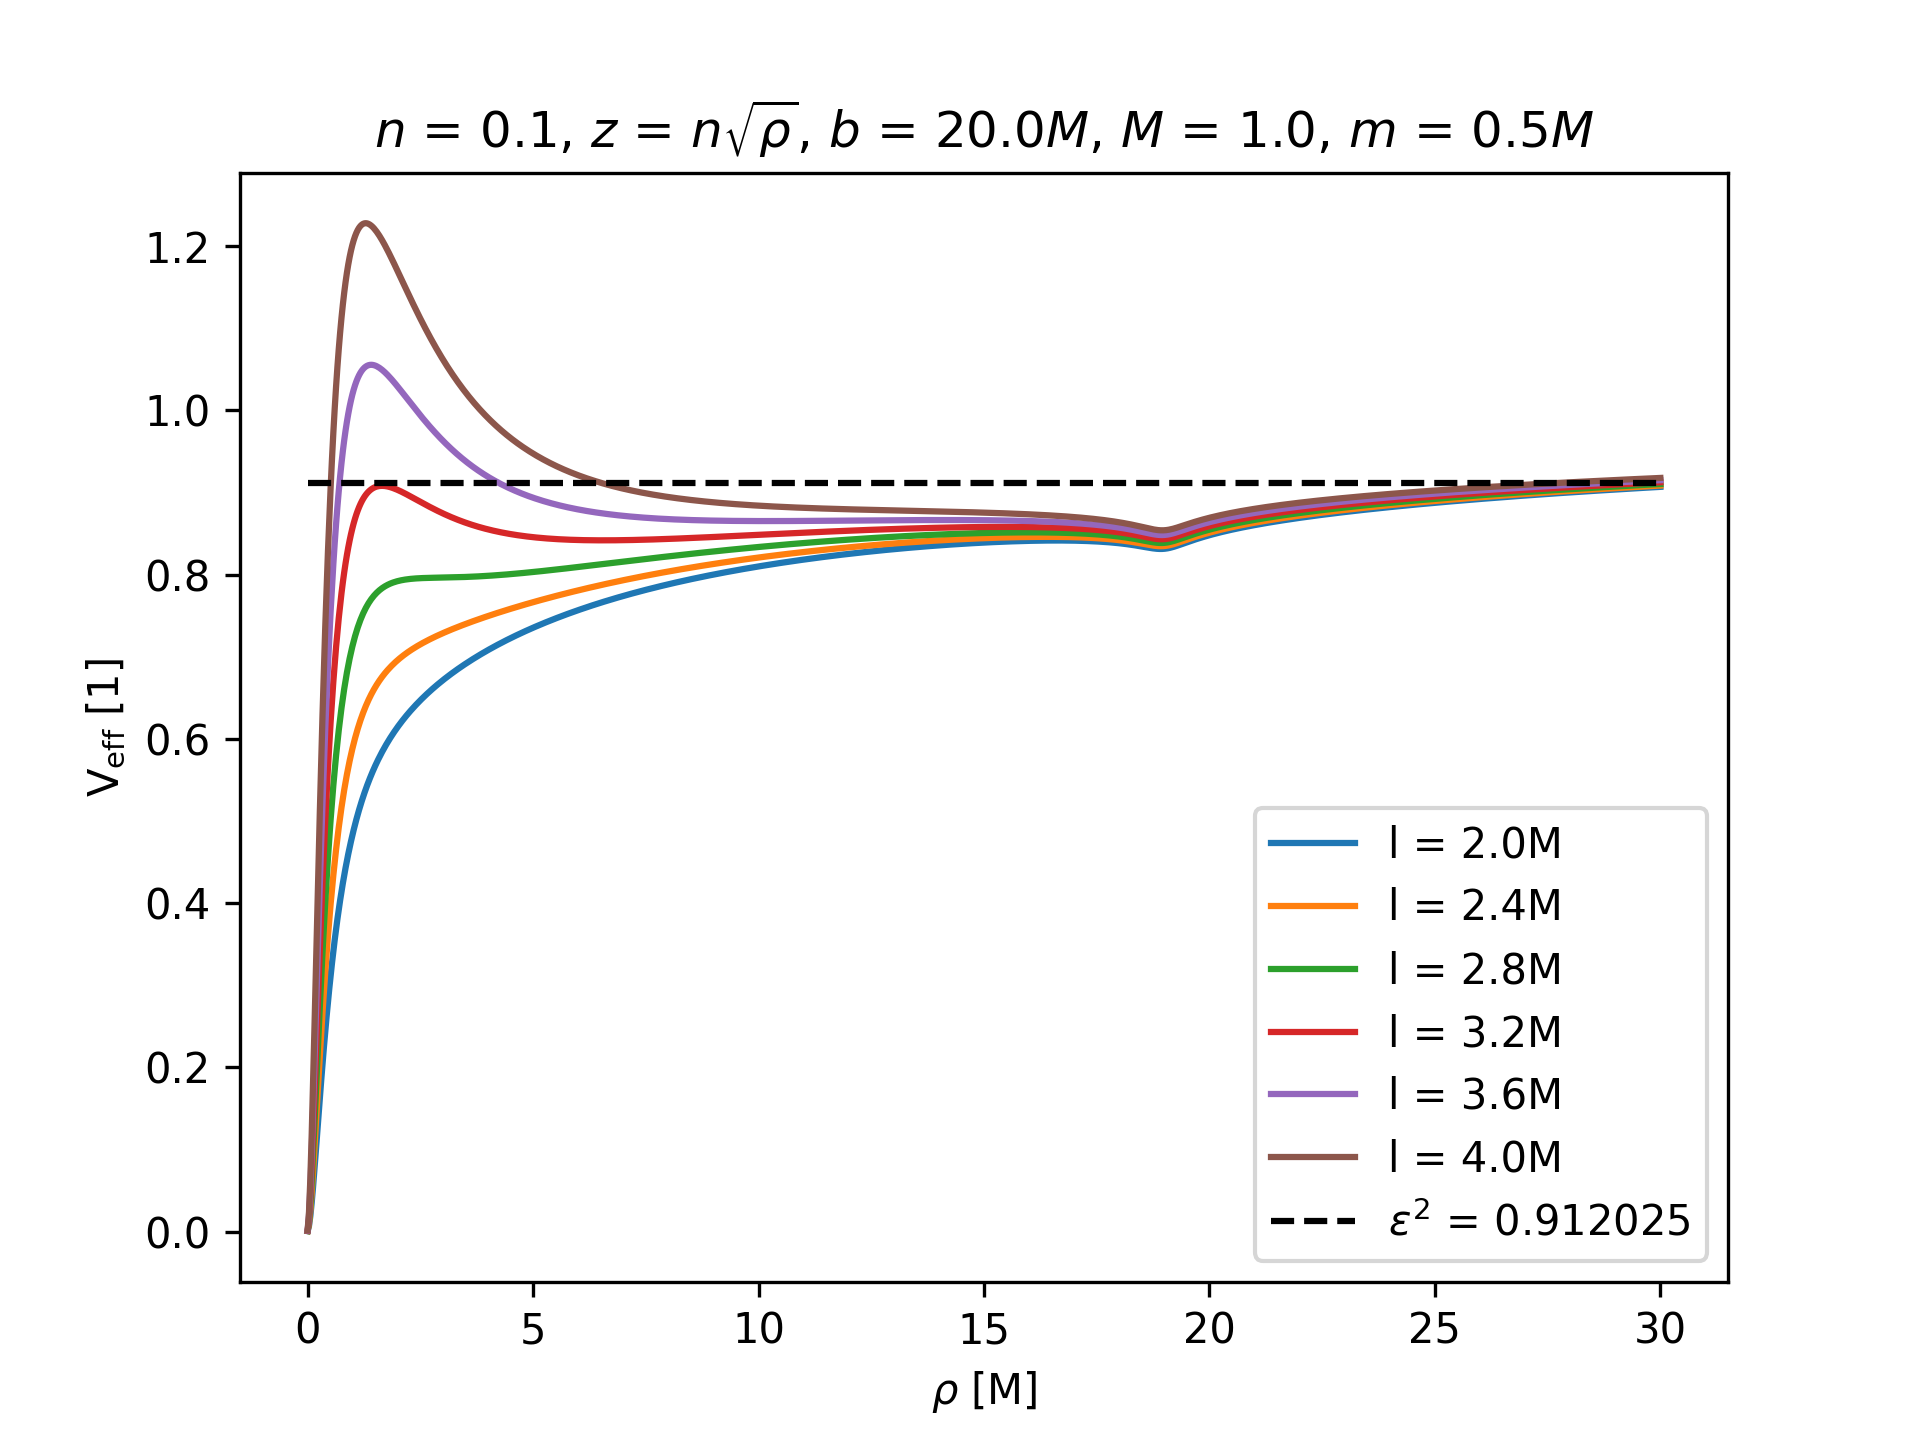
\includegraphics[width=0.82\linewidth]{img/rn_mp_Veff.png}
    \caption{Effective potential \(V_{\mathrm{ef}}\) of the RN+MP system for \(z(\rho)=n\sqrt{M\rho}\), with \(n=0.1\), \(M=1\), \(\mathcal{M}=0.5M\), \(b=20M\), and several values of \(l\). The horizontal dashed line marks \(\epsilon^2\) for \(\epsilon=0.955\).}
    \label{fig:rn-mp-veff-z-of-rho}
\end{figure}

\begin{figure}[H]
    \centering
    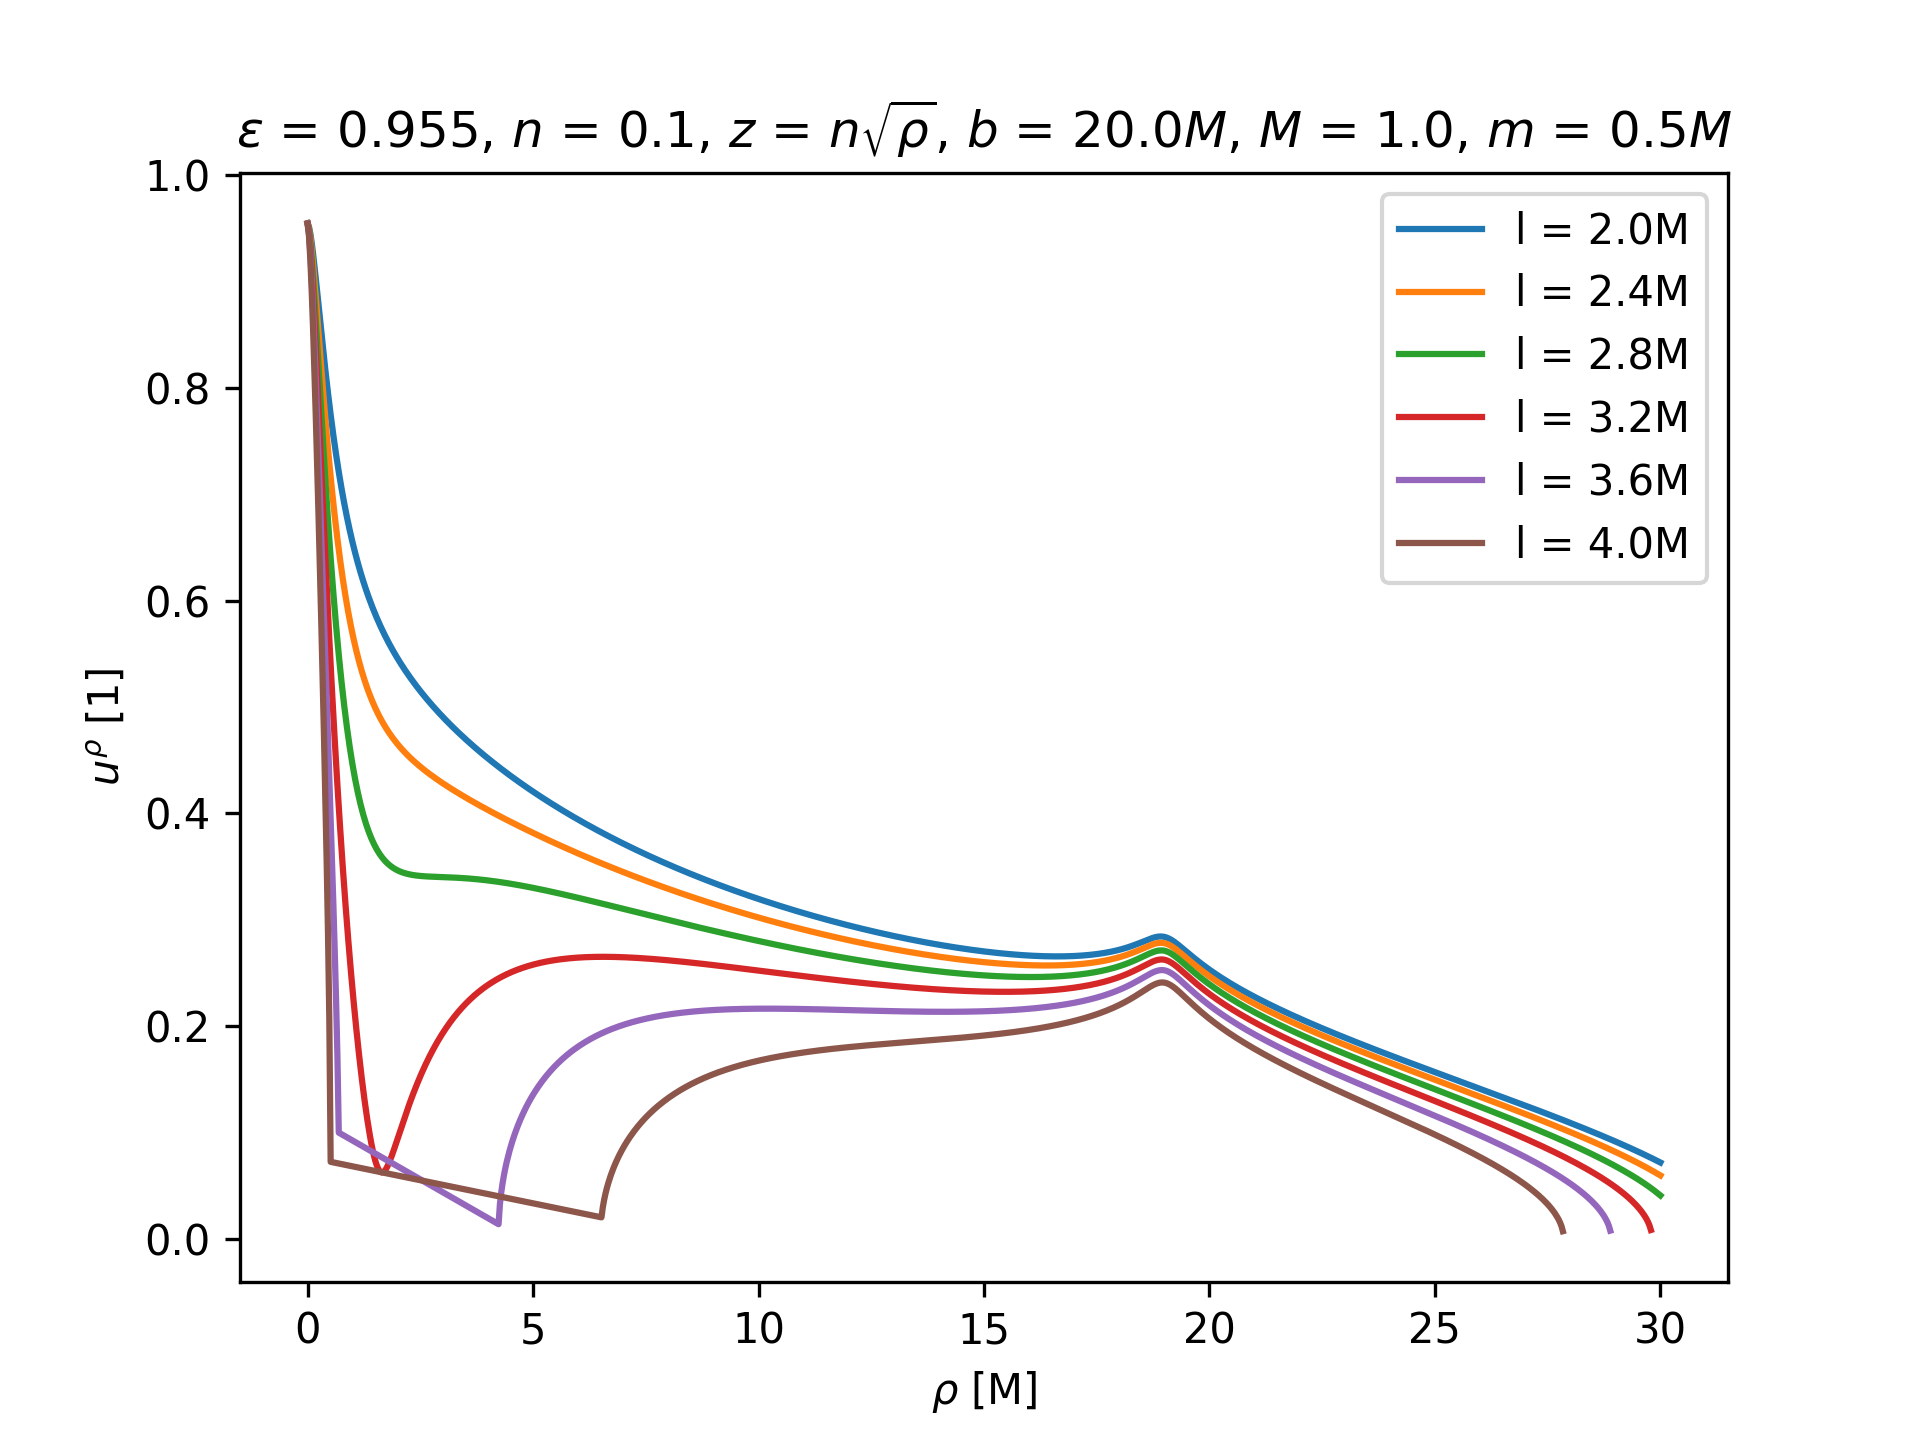
\includegraphics[width=0.82\linewidth]{img/rn_mp_accessible_region.png}
    \caption{Accessible region of the RN+MP system for \(z(\rho)=n\sqrt{M\rho}\), with \(n=0.1\), \(M=1\), \(\mathcal{M}=0.5M\), \(b=20M\), \(\epsilon=0.955\), and several values of \(l\). The plotted curves give the positive branch of \(u^\rho_{\mathrm{MAX}}\).}
    \label{fig:rn-mp-accessible-z-of-rho}
\end{figure}

With this choice of \(z(\rho)\), the accessible region opens towards the
horizon. For some values of the parameters it can still be separated into
disconnected components, and a trajectory starting in one component cannot cross
into another. For the RN+MP basin maps we therefore choose energies slightly
above the local maximum of \(V_{\mathrm{ef}}\) associated with the unstable
circular orbit, so that the selected accessible region is connected while still
sampling the neighbourhood of the former separatrix. The corresponding
trajectories are not exact homoclinic trajectories; rather, they lie near the
perturbed homoclinic structure. The Melnikov analysis of the RN+MP system by
Polcar and Semer\'ak~\cite{PolcarSemerak2019}, building on the homoclinic
mechanism discussed in Section~\ref{sec:homoclinic-tangles}, shows that the
stable and unstable manifolds split and intersect transversely. We therefore
expect the richest basin boundaries when the sampled initial conditions lie near
this separatrix-derived chaotic layer.

\subsection{Heuristic}
Now we shall discuss how to construct the basin map and how to calculate the
fractal dimension of the basin boundary. In order to construct a basin map, we
need to solve a large number of trajectories for different initial conditions.
For this we use the Gravitacek 2 solver written in C++ by Karel Kraus~\cite{Kraus2025},
with minor modifications made for this thesis. The solver is available at
\url{https://github.com/ImmanuelKant314/Gravitacek-2}, and the thesis code is
available at \url{https://github.com/DJopek/chaos}. For a given set of
parameters \(M\), \(\mathcal{M}\), \(b\), \(\sigma\), \(\epsilon\), \(l\), and
\(T_{\mathrm{MAX}}\), we construct a basin map in the
\((\rho_0,u^\rho_0)\) plane. Here \(b\) is the Schwarzschild or
Reissner--Nordstr\"om radial coordinate used to specify the ring radius, while
\(\sigma\) is the corresponding Weyl or Majumdar--Papapetrou cylindrical radius
defined in Eqs.~\eqref{eq:schw-bw-ring-radius} and
\eqref{eq:rn-mp-ring-radius}. The computational grid contains \(N\times N\)
initial conditions; each coloured cell corresponds to one integrated trajectory.

The colour assignment is a numerical final-state proxy. The solver checks
conservation of \(\epsilon\) and \(l\), stopping if the relative error exceeds
\(10^{-10}\) for SCHW+BW trajectories and \(10^{-9}\) for RN+MP trajectories.
It also stops when the trajectory approaches the black hole or the ring too
closely. The code uses \texttt{long double}; the actual precision depends on the
compiler and architecture. The integration method is Dormand--Prince 853, an
eighth-order Runge--Kutta scheme with embedded lower-order estimates for step
control.

If a trajectory stops before \(T_{\mathrm{MAX}}\), we colour the corresponding
initial condition light blue and label it as a plunge/termination outcome. This
class includes physical approaches to singular parts of the geometry, but it can
also include trajectories for which the conservation-error event stopped the
integration. If a trajectory survives until \(T_{\mathrm{MAX}}\), we colour it
dark blue and label it as an eternal-orbit outcome. Initial conditions outside
the accessible region are coloured white and are not treated as a physical
outcome basin. For the uncertainty-exponent calculation we use selected windows
inside the accessible region and perturb the \(\rho_0\) coordinate by
\(\varepsilon=10^{-4},10^{-3},10^{-2}\), as described in
Section~\ref{sec:uncertainty-exponent}. The fitted uncertainty exponent
\(\alpha\) then gives the two-dimensional basin-boundary estimate \(d=2-\alpha\).
